\chapterA{Hito 2 - Fase de Modelado}
\section{Listado de factoides}
El listado de factoides es el producto resultado de la fase de investigación. Para obtenerlo se ha extraído las principales características de las
diversas entrevistas, de todas las respuestas a los cuestionarios y del análisis de la competencia. Respecto a los obtenidos en el anterior hito,
hemos realizado una serie de cambios debido a la falta de respuestas a algunas de las variables que hemos identificado y a los problemas que se
han podido identificar durante la corrección de dichos factoides.


Tras la corrección del hito anterior y observando las necesidades del diseño de personas de este hito, vamos a realizar una serie de modificaciones
en la lista de factoides, reflejando los cambios que han sido realizados con la letra en cursiva. Cabe destacar que el usuario Alberto ha sido finalmente
descartado debido a que sus características no se encuadraban dentro de las propuestas en la hipótesis de usuarios y los factoides de Sofía y la competencia se han hecho de nuevo. \\

\textbf{Factoides de Madi:}

\begin{itemize}
    \item Madi es secretaria de la FEDDI y lleva 16 años trabajando allí.
    \item Madi se encarga de organizar los viajes cuadrando horarios y comprando billetes.
    \item Madi compra billetes a través de Renfe, Air Europa o Iberia porque le sale más económico que en un comparador.
    \item Madi se encarga de los viajes de campeonatos internacionales que les recepciona, les recoge y les lleva al punto de encuentro.
    \item Madi ve que el problema principal para los deportistas es la dependencia de sus padres y entrenadores, el manejo de las aplicaciones y el internet y para algunos necesitan acompañante.
    \item Madi considera que necesitan acompañantes porque tienen problemas para orientarse y no se manejan bien.
    \item Para Madi las dificultades dependen mucho del grado de discapacidad.
    \item Madi no usa aplicaciones, sólo compra en páginas oficiales de la aerolínea.
    \item Madi utiliza la agencia de viajes Betravel para vuelos internacionales.
    \item Madi descarta Ryanair.
    \item Madi no utiliza comparadores porque ya tiene localizadas dos compañías y Renfe que ofrecen el servicio de acompañamiento de AENA.
    \item Madi tiene en cuenta el precio y la variedad de horarios para coger un billete.
    \item Madi no se fija en más facilidades, esos son los atletas.
    \item Madi considera que el comparador debe ser muy simple (lugar, destino y fecha).
    \item A Madi le parece importante que se pueda ver qué tipos de servicios de acompañantes ofrecen.
    \item \textit{En los campeonatos de España son los clubes los encargados del desplazamiento de los deportistas (ella no interviene)}.
\end{itemize}


\textbf{Factoides de Sofia:}

\begin{itemize}
    \item \textit{Sofía es estudiante, tiene 21 años y considera que tiene un buen manejo de la tecnología.}
    \item \textit{A Sofia le gusta viajar y considera que es uno de sus hobbies favoritos porque le gusta conocer nuevas culturas, vivir experiencias y explorar lugares desconocidos.}
    \item \textit{Sofía ha viajado por Europa, Estados Unidos y por el territorio nacional.}
    \item \textit{A Sofia le gustaría viajar más.}
    \item \textit{Sofía usa distintos métodos de transporte como coche, transporte público, avión, tren, bus y privado, este último rara vez.}
    \item \textit{Sofía prefiere usar autobuses solo cuando viaje distancias cortas o medias.}
    \item \textit{Sofía normalmente suele viajar con amigos y familiares por ocio.}
    \item \textit{Sofía no recuerda haber tenido ningún problema viajando, aunque admite que cuando viaja lo hace con la mente más abierta de lo que la tiene normalmente.}
    \item \textit{Sofía a veces organiza los viajes que hace y a veces no.}
    \item \textit{Sofía busca viajes económicos y que se adapten a sus necesidades.}
    \item \textit{Sofia utiliza varios comparadores de viajes a la hora de organizar un viaje para buscar las mejores ofertas. Por ejemplo: Kayak, Skyscanner, Trivago.}
    \item \textit{A Sofía le gustaría que los comparadores de viajes mostraran el precio final del billete, con los posibles extras incluidos, piensa que es un punto a mejorar.}
    \item \textit{Sofía prefiere usar aplicaciones web a aplicaciones móviles, y suele hacer estas gestiones desde el ordenador.}
    \item \textit{Sofía piensa que algunos comparadores son tediosos a la hora de usar ya que algunos tardan mucho en cargar o te redirigen a otra páginas.}
    \item \textit{Cuando Sofía ha tenido problemas con algún comparador ha optado por usar otro comparador que no tuviera esos problemas.}
    \item \textit{Sofía considera que con una interfaz sencilla y fácil de usar sería suficiente para un comparador.}
    \item \textit{Sofía considera que los comparadores de viajes son bastante accesibles, pero que quizás aclarar algunas cosas en las webs o los anuncios de spam en las webs pueden molestar a personas con discapacidad intelectual.}
    
\end{itemize}

\textbf{Factoides de Beatriz:}
\begin{itemize}
    \item Beatriz tiene 21 años.
    \item Beatriz se desenvuelve bien con las tecnologías y declara usarlas a diario.
    \item \textit{Beatriz viaja por ocio, para conocer nuevos lugares y culturas o visitar familiares.}
    \item Beatriz viaja una vez al año, sobre todo dentro de España, y fuera de España una vez cada dos años.
    \item \textit{A Beatriz le gustaría viajar más porque viaja poco para su gusto y salir de España más de una vez al año, los motivos por los que no puede hacerlo con más frecuencia es por su situación económica y el escaso tiempo que tiene de vacaciones.}
    \item Suele viajar en coche o en avión para distancias más largas.
    \item Beatriz suele viajar para visitar a familiares o por razones de ocio.
    \item Beatriz suele viajar acompañada (normalmente de sus familiares).
    \item Cuando viaja con su familia, organizan el viaje conjuntamente.
    \item \textit{En los próximos meses viajará al extranjero para ver a su pareja.}
    \item \textit{Beatriz prioriza el precio del billete.}
    \item Cuando no viaja con su familia, Beatriz suele organizar los viajes que hace.
    \item Beatriz se fija sobretodo en el precio a la hora de tomar una decisión, por ejemplo, para comprar un vuelo.
    \item En su último viaje, Beatriz optó por usar una aplicación (eDreams) debido a que tenían un programa con prueba gratuita con el que sus vuelos le salieron más baratos.
    \item Beatriz prefiere los vuelos de ida tempranos y los de vuelta más tarde.
    \item A la hora de hacer la reserva, Beatriz cree que lo más tedioso son todas las pantallas que tienes que atravesar en las que te ofrecen todo tipo de servicios extra, alguno incluso ofreciéndose dos veces.
    \item A Beatriz también le gustaría que los comparadores pusieran un mensaje más claro en el caso de que ida y vuelta sean desde aeropuertos distintos.
    \item Google es su navegador favorito, principalmente porque lo lleva usando mucho tiempo y está acostumbrada, pero también debido a la conectividad con otros servicios en su móvil y porque considera que es lo mejor en cuanto a desarrollo web; también le gusta su estética.
    \item El comparador favorito de vuelos de Beatriz es el comparador de Google u otros.
    \item Beatriz considera que los comparadores de vuelos pueden no ser accesibles para personas que no tengan mucha soltura con las tecnologías.
    \item Beatriz considera que eDreams es muy estético, más que el comparador de Google o que otros.
    \item \textit{Para ella no es un problema sacrificar facilidades como el tipo y la cantidad de equipaje, la elección de asiento o los horarios de ida y vuelta para que el precio sea más barato}.
    \item \textit{Beatriz destaca también que al comprar en eDreams tuvo un problema con la aerolínea, lo que la llevó a tener que pasar un proceso poco accesible y con más cargos económicos.}
    \item \textit{Beatriz destaca que generalmente prefiere hacer estas reservas de viajes en el ordenador en vez de en el móvil.}
\end{itemize}


\textbf{Factoides del cuestionario:}

\begin{itemize}
    \item La mitad de los usuarios tienen entre 19 y 25 años y la otra mitad entre 26 y 65 años.
    \item La mayoría de los encuestados viven en la ciudad, pocos en pueblos.
    \item Dos tercios de los encuestados tienen un poder adquisitivo medio. Un tercio, bajo y muy pocos, alto.
    \item La mayoría de los encuestados les gusta viajar, pocos no.
    \item La mayoría de los encuestados le gusta viajar por conocer nuevos lugares y los pocos que no, es por la gente o por no parar de moverse.
    \item La mayoría de los encuestados viajan al menos una vez al año, el resto viajan al menos una vez al mes y muy poco no viajan.
    \item La mayoría de los encuestados le gustaría viajar más, el resto no.
    \item Todos los encuestados disfrutan cuando viajan.
    \item Los medios de transporte que usan los encuestados son coche propio, transporte público y aéreo.
    \item Los encuestados suelen viajar por ocio, pocos por trabajo.
    \item Las herramientas que más utilizan los encuestados son Trivago, Kayak y SkyScanner. Hay un tercio de los encuestados que no usan ninguna.
    \item Los comparadores de viajes (Trivago, Kayak, Rastreator, SkyScanner, Momondo) son de fácil uso.
    \item Un quinto de los encuestados tienen alguna discapacidad reconocida.
    \item Los encuestados con discapacidad la mayoría tienen discapacidad física y el resto es intelectual o mental.
    \item Los encuestados con discapacidad dos tercios necesitan adaptaciones para sus viajes como para sillas de ruedas.
    \item La mayoría de los encuestados con discapacidad a veces planifican y el resto o nunca o siempre.
    \item Un tercio de los encuestados con discapacidad encuentran dificultad en el proceso de búsqueda por la accesibilidad.
    \item La mayoría de los encuestados con discapacidad no les supone una dificultad buscar medio de transporte, hacer, comparar y ver las ventajas/desventajas de las rutas o comparar precios.
    \item La mitad de los encuestados con discapacidad no usan comparadores de viajes o similares.
    \item Los encuestados con discapacidad que han usado comparadores la mayoría ha desistido.
    \item Para los encuestados con discapacidad les parece complejo solicitar ayuda dentro de la aplicación de viajes.
    \item La inmensa mayoría de los encuestados sin discapacidad ha viajado en el último año.
    \item La mayoría de los encuestados sin discapacidad hace búsqueda de viaje.
    \item Dos tercio de los encuestados sin discapacidad han utilizado un comparador de viajes.
    \item El motivo principal de los encuestados sin discapacidad es ahorrar dinero. También está mayor oferta, facilidad de uso y ahorra tiempo.
    \item Los encuestados sin discapacidad no tienen problemas con los comparadores.
    \item A los encuestados sin discapacidad les supone una dificultad en el tema de la accesibilidad tener que hacer muchas operaciones para llegar a un objetivo.
    \item Los encuestados están de acuerdo en su mayoría de que está bien la accesibilidad salvo por la ausencia de ayudas al rellenar.
    \item La mayoría de los encuestados no ha echado en falta ninguna funcionalidad.
\end{itemize}


\textbf{Factoides del análisis de competencia}

\begin{itemize}
    \item \textit{Todas las aplicaciones ofrecen como mínimo poder buscar vuelos, algunas incluyen trenes y buses en las búsquedas.}
    \item \textit{Las funcionalidades buscadas en otras aplicaciones son búsqueda de medio de transporte, comparar precios para el mismo viaje, y comprar billetes.}
    \item \textit{Todas las aplicaciones tienen un sistema de opiniones y de valoración con estrellas.}
    \item \textit{Todas las páginas que ofrecen servicio de comparar transporte tienen buenos filtros de búsqueda.}
    \item \textit{Todas ofrecen como mínimo poder buscar vuelos, algunas incluyen trenes y buses en las búsquedas.}
    \item \textit{Casi todas ofrecen un sistema de seguros a la hora de comprar un medio de transporte.}
    \item \textit{Solo dos de las páginas estudiadas ofrecen opciones de ecologismo.}
    \item \textit{En los autobuses no es hasta el final de la reserva donde se puede designar que el cliente es una persona con discapacidad física.}
    \item \textit{En trenes al principio te deja marcar la casilla “Trenes con plaza H”, la cual es una plaza habilitada para personas con discapacidad física que necesitan una silla de ruedas.}
    \item \textit{A la hora de realizar el pago puedes marcar la “tarjeta dorada”, la cual aplica un descuento para personas con discapacidad.}
    \item \textit{En los servicios de reserva de autobuses no es hasta el final de la reserva cuando se puede marcar que el cliente es una persona con discapacidad física.}
    \item \textit{No todas ofrecen poder buscar con flexibilidad de fechas.}
\end{itemize}

\section{Modelado}
La fase de modelado es la segunda etapa del proceso de Diseño Guiado por Objetivos (DGO). En esta fase, partiremos de la lista de factoides que
obtuvimos en la etapa anterior y con ella diseñar los prototipos de personas que serán los potenciales usuarios de la misma, representando además
las principales características que extrajimos de los factoides.

Para poder lograr este objetivo, vamos a utilizar el proceso de diseño de personas bottom-up propuesto por Copper, que consta de las siguientes fases:
\begin{itemize}
    \item \textbf{Identificación de variables de comportamiento} $\rightarrow$ El primer paso que vamos a seguir es identificar las distintas variables de comportamiento que vamos a tener en la lista de factoides y ver los posibles valores que van a tomar.
    \item \textbf{Relación de individuos con las variables de comportamiento} $\rightarrow$ Tras haber identificado las variables, vamos a ver para cada uno de los usuarios entrevistados el valor que van a tomar cada una de ellas en base a los factoides obtenidos.
    \item \textbf{Identificación de patrones de comportamiento} $\rightarrow$ Una vez configurada la matriz que relaciona los usuarios con las variables, vamos a marcar en ella las posibles repeticiones que aparezcan para poder establecer un listado de patrones de comportamiento con los que vamos a realizar los esqueletos de las personas.
    \item \textbf{Creación de esqueletos} $\rightarrow$ Tras haber identificado los distintos patrones de comportamiento, vamos a crear los esqueletos que nos van a servir de plantilla para las personas definitivas que vamos a desarrollar en los siguientes apartados.
    \item \textbf{Revisión de la completitud y la redundancia} $\rightarrow$ Cuando los esqueletos de las personas ya estén finalizados, el siguiente paso es comprobar su completitud y evitar posibles redundancias entre ellos, haciendo que todas las personas que se representen tengan todos los factoides y se eviten repeticiones entre ellas.
    \item \textbf{Elaboración de las personas} $\rightarrow$ Al finalizar la revisión de los esqueletos, lo siguiente que ha de hacerse es desarrollar las personas a partir de ellos, dando los principales motivos y acciones que llevan a cada una de ellas.
    \item \textbf{Validación de las personas} $\rightarrow$ Para poder validar las personas, tenemos que cerciorarnos de que representen todos y cada uno de los factoides que tenemos, tanto los de las entrevistas como los de los cuestionarios y el análisis de la competencia.
    \item \textbf{Tipos de las personas} $\rightarrow$ Por último, cuando ya se tienen validadas todas las personas elaboradas, vamos a decir en base a las características que presentan, el tipo de persona ante el que nos encontramos.
\end{itemize}

\subsection{Planificación del hito}
Para poder planificar este hito correctamente, hemos identificado en una Hoja de cálculo (ver figura \ref{fig:planif-hito2}) las distintas tareas que tenemos que 
realizar, junto al intervalo de fechas en el que se encuentra prevista su realización y el / los responsables de dicha tarea.

\begin{figure}[H]
    \centering 
    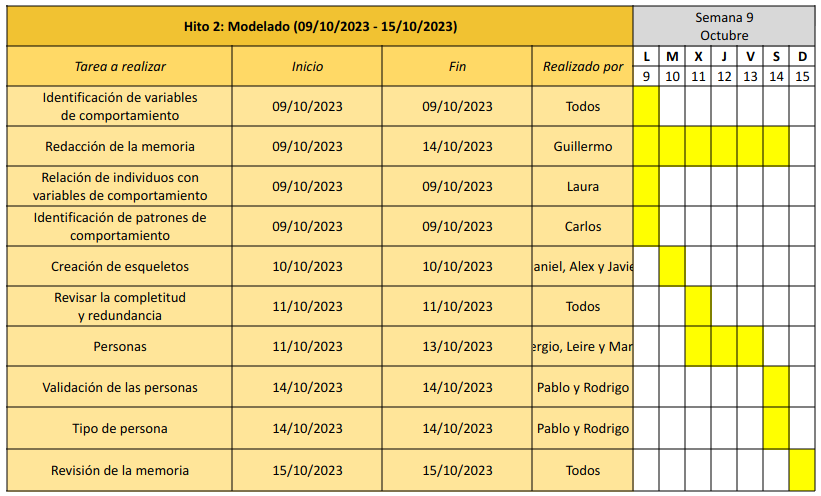
\includegraphics[width=0.5\textwidth]{./Imagenes/Planificaciones/Planif-hito2.png}
    \caption{Planificación Hito 2}
    \label{fig:planif-hito2}
\end{figure}

\subsection{Identificación de variables de comportamiento}
En la fase de modelado, el primer paso que debemos seguir es la identificación de las variables de comportamiento. 
Estas variables van a ser producto de las listas de factoides que confeccionamos durante el hito anterior y hemos 
corregido antes de comenzar a trabajar en este. El proceso de confección de las variables consiste en identificar 
posibles características que pueden encasillar a los usuarios y a partir de ellas darles un rango de valores que 
podamos asignar a nuestros usuarios. Las variables que hemos podido identificar (y sus valores) son las siguientes:
\begin{itemize}
    \item \textbf{Rango de edad} (18- / 18 - 25 / 26 - 40 / 40 - 65 / 65+) $\rightarrow$ Intervalo de edad en el que se encuentra la persona que estamos analizando.
    \item \textbf{Estado civil} (Casad@ / En pareja / Solter@) $\rightarrow$ Condición de una persona en relación con su nacimiento, nacionalidad, filiación o 
    matrimonio, que se hacen constar en el registro civil y que delimitan el ámbito propio de poder y responsabilidad que el derecho reconoce a las personas naturales.
    \item \textbf{Organización de viajes} (Sí / No) $\rightarrow$ Indica si la persona ha realizado o no la reserva de un viaje, pasando por todas sus etapas hasta que
    haya finalizado.
    \item \textbf{Uso de comparadores de viajes} (Sí / No) $\rightarrow$ Define si la persona, en su proceso de búsqueda y reserva de viajes, ha utilizado o no como
    herramienta un comparador de viajes para buscar las mejores ofertas.
    \item \textbf{Frecuencia de viaje} (Baja / Media / Alta) $\rightarrow$ La frecuencia con la que la persona suele viajar. Definimos frecuencia baja como una vez al año
    o menos, media como 3-4 veces al año y alta más de estas cifras.
    \item \textbf{Tipo de viaje} (Ocio / Trabajo / Estudios) $\rightarrow$ Indica el motivo por el que se realiza el viaje. Ocio es si viaja por gusto, trabajo si se tiene que desplazar para tener que trabajar y estudios entendemos movilidad, es decir, Erasmus y programas derivados.
    \item \textbf{Discapacidad} (Sí / No) $\rightarrow$ Indica si el usuario presenta alguna discapacidad. En caso afirmativo, se presenta también el tipo de discapacidad que presenta.
    \item \textbf{Acompañante} (Familia / Amigos / Pareja / Solo) $\rightarrow$ Persona(s) con las que suele viajar el usuario. En caso de que lo haga con varios de los grupos presentes, se selecciona con el que lo haga con más frecuencia.
    \item \textbf{Medio de transporte más frecuente} (Avión / Tren / Vehículo propio / Transporte público / Otro) $\rightarrow$ Medio de transporte que utiliza el usuario con mayor frecuencia. Al igual que en el caso anterior, en caso de seleccione varios, se tomará en cuenta la preferencia directa del usuario.
    \item \textbf{Uso de tecnología} (Bajo / Medio / Alto) $\rightarrow$ Denota la facilidad con la que la persona se entiende con la tecnología. Si es bajo, indica que sus conocimientos con básicos, mientras que si es alto indica un nivel de manejo muy avanzado.
    \item \textbf{Viaje nacional} (Sí / No) $\rightarrow$ Define si el usuario ha realizado viajes por el territorio nacional (España) o si no lo ha hecho.
    \item \textbf{Viaje internacional} (Sí / No) $\rightarrow$ Indica si el usuario ha realizado viajes fuera del territorio nacional o si no lo ha hecho
    \item \textbf{Trabaja} (Sí / No) $\rightarrow$ Indica la situación laboral del usuario, es decir, si actualmente trabaja o no.
    \item \textbf{Gusto por viajar} (Sí / No) $\rightarrow$ Denota si el usuario disfruta cuando viaja o si bien no es agradable para él el hecho de viajar y lo hace por obligación.
    \item \textbf{Nivel de ahorro} (Bajo / Medio / Alto) $\rightarrow$ Indica el nivel de ahorro que tiene el usuario. Definimos bajo como una escasa capacidad para ahorrar y alto como una buena capacidad de ahorro.
\end{itemize}

\subsection{Relación de individuos con variables de comportamiento}
Tras haber identificado las variables de comportamiento en la fase anterior, vamos a ver para cada uno de los usuarios entrevistados (en base a los factoides
que tenemos registrados) los valores que van a tomar en cada una de ellas. Para mostrar estos resultados vamos a realizar una matriz (ver cuadro \ref{table:relacion-individuos-variables})
en la que vamos a enfrentar cada una de las variables con los entrevistados, poniendo en cada celda el valor que va a tomar la variable para dicho usuario.
\begin{table}[H]
    \centering
    \begin{tabular}{|p{10em}|p{7em}|p{7em}|p{7em}|p{8em}|}
        \hline
        \cellcolor{black}                 & \cellcolor{black}{\textcolor{white}{Madi}}  & \cellcolor{black}{\textcolor{white}{Sofía}}   & \cellcolor{black}{\textcolor{white}{Beatriz}} \\ \hline
        Rango de edad                     &                                             & 18 - 25                                       & 18 - 25                                       \\ \hline
        Estado civil                      &                                             & Soltera                                       & En pareja                                     \\ \hline
        Organización de viajes            & Si                                          & Si                                            & Si                                            \\ \hline
        Uso de comparadores de viajes     & No                                          & Kayak, Skyscanner, Trivago                    & eDreams, comparador de Google                 \\ \hline
        Frecuencia de viaje               & Alta                                        & Media                                         & Baja                                          \\ \hline
        Tipo de viaje                     & Trabajo                                     & Ocio                                          & Ocio                                          \\ \hline
        Discapacidad                      & No                                          & No                                            & No                                            \\ \hline
        Acompañante                       &                                             & Familia                                       & Familia                                       \\ \hline
        Medio de transporte más frecuente &                                             & Transporte público                            & Vehículo propio                               \\ \hline
        Uso de tecnología                 &                                             & Alto                                          & Alto                                          \\ \hline
        Viaje nacional                    & Si                                          & Si                                            & Si                                            \\ \hline
        Viaje internacional               & Si                                          & Si                                            & Si                                            \\ \hline
        Trabaja                           & Si                                          & No                                            & No                                            \\ \hline
        Gusto por viajar                  &                                             & Si                                            & Si                                            \\ \hline
        Nivel de ahorro                   & Alto                                        & Alto                                          & Alto                                          \\ \hline
    \end{tabular}
    \caption{Matriz de relación de los individuos con las variables de comportamiento}
    \label{table:relacion-individuos-variables}
\end{table}

Una vez construida la matriz que relaciona los individuos con las variables, vamos a justificar las razones por las cuáles hemos asignado un
determinado valor a las variables para cada uno de los usuarios. \\

\noindent Justificación de las variables de Madi:
\begin{itemize}
    \item \textbf{Rango de edad} $\rightarrow$ No lo ha comentado.
    \item \textbf{Estado civil} $\rightarrow$ No lo ha comentado.
    \item \textbf{Organización de viajes} (Si) $\rightarrow$ “Madi se encarga de organizar los viajes cuadrando horarios y comprando billetes.”
    \item \textbf{Uso de comparadores de viajes} (No) $\rightarrow$ “Madi no utiliza comparadores porque ya tiene localizadas dos compañías y Renfe que ofrecen el servicio de acompañamiento de AENA.”
    \item \textbf{Frecuencia de viaje} (Alta) $\rightarrow$ “Madi se encarga de los viajes de campeonatos internacionales que ella les recepciona, les recoge y les lleva al punto de encuentro. Madi comenta que hay bastantes campeonatos.” Porque al menos asiste a los viajes internacionales que pueden ser no muy frecuentes.
    \item \textbf{Tipo de viaje} (Trabajo) $\rightarrow$ Se encarga de los viajes de su trabajo y viaja por ello.
    \item \textbf{Discapacidad} (No) $\rightarrow$ Se deduce porque trabaja en una federación y organiza viajes para gente con discapacidad.
    \item \textbf{Acompañante} $\rightarrow$ No lo ha comentado, podría ser sus compañeros de trabajo.
    \item \textbf{Medio de transporte más frecuente} $\rightarrow$ no se sabe realmente, podría ser avión o tren.
    \item \textbf{Uso de la tecnología} $\rightarrow$ tampoco lo comenta, sólo el de los deportistas.
    \item \textbf{Viaje Nacional} (Si) $\rightarrow$ “Madi comenta que en los campeonatos de españa, los clubes son los encargados del desplazamiento de los deportistas, ella interviene poco o nada.” eso significa que el poco puede llegar a viajar en algún momento en los nacionales.
    \item \textbf{Viaje internacional} (Si) $\rightarrow$ “Madi se encarga de los viajes de campeonatos internacionales que ella les recepciona, les recoge y les lleva al punto de encuentro. Madi comenta que hay bastantes campeonatos.”, recoge a los deportistas por lo que hace el viaje.
    \item \textbf{Trabaja} (Si) $\rightarrow$ “Madi es secretaria de la FEDDI y lleva 16 años trabajando allí.”
    \item \textbf{Gusto por viajar} $\rightarrow$ No lo ha dicho.
    \item \textbf{Nivel de Ahorro} (Alto) $\rightarrow$ “Madi compra billetes a través de Renfe, Air Europa o Iberia porque le sale más económico que en un comparador.” suponemos que escoge lo más económico para ahorrar lo máximo posible.
\end{itemize}

\noindent Justificación de las variables de Sofía:
\begin{itemize}
    \item \textbf{Rango de edad} (18 - 25) $\rightarrow$ “Sofía tiene 21 años.”
    \item \textbf{Estado civil} (Soltero) $\rightarrow$ No lo ha comentado, pero parece no tener pareja. 
    \item \textbf{Organización de viajes} (Si) $\rightarrow$ “Sofía a veces organiza los viajes que hace y a veces no.”
    \item \textbf{Uso de comparadores de viajes} (Kayak, Skyscanner, Trivago) $\rightarrow$ “Sofía utiliza varios comparadores de viajes a la hora de organizar un viaje. Por ejemplo: Kayak, Skyscanner, Trivago.”
    \item \textbf{Frecuencia de viaje} (Media) $\rightarrow$ “Sofía viaja a menudo, tanto fuera como dentro de España.”, a menudo será lo normal.
    \item \textbf{Tipo de viaje} (Ocio) $\rightarrow$ “Sofía ha hecho viajes de varios tipos. Desde intercambios lingüísticos a viajes familiares o con amigos, para conocer nuevas ciudades o relajarse.”
    \item \textbf{Discapacidad} (No) $\rightarrow$ “Sofía considera que los comparadores de viajes son bastante accesibles, pero que quizás aclarar algunas cosas en las webs o los anuncios de spam en las webs pueden molestar a personas con discapacidad intelectual.” da a intuir que ella no tiene discapacidad.
    \item \textbf{Acompañante} (Familia) $\rightarrow$ “A Sofía le gusta ir alternando entre viajar sola, con familia o con amigos, disfruta de todas.” Más con familia ya que es estudiante y no tiene trabajo para pagar tantos viajes.
    \item \textbf{Medio de transporte más frecuente} (Transporte público) $\rightarrow$ “Sofía usa tanto automóviles como trenes y autobuses en sus viajes dependiendo del sitio al que viaje.” “Sofía prefiere usar autobuses solo cuando viaje distancias cortas o medias” En cualquiera de los dos casos incluye transporte público.
    \item \textbf{Uso de la tecnología} (Alto) $\rightarrow$ “Sofía tiene 21 años y considera que tiene un buen manejo de la tecnología”
    \item \textbf{Viaje Nacional} (Si) $\rightarrow$ “Sofía viaja a menudo, tanto fuera como dentro de España.”
    \item \textbf{Viaje internacional} (Si) $\rightarrow$ “Sofía viaja a menudo, tanto fuera como dentro de España.”
    \item \textbf{Trabaja} (No) $\rightarrow$ “Sofía es estudiante, tiene 21 años y considera que tiene un buen manejo de la tecnología” 
    \item \textbf{Gusto por viajar} (Si) $\rightarrow$ “A Sofía le gusta viajar y desde pequeña ha querido conocer las diferentes partes del mundo.”
    \item \textbf{Nivel de Ahorro} (Alto) $\rightarrow$ “Sofía busca viajes económicamente accesibles.” quiere ahorrar lo máximo posible.
\end{itemize}

\noindent Justificación de las variables de Beatriz:
\begin{itemize}
    \item \textbf{Rango de edad} (18 - 25) $\rightarrow$ “Beatriz tiene 21 años.”
    \item \textbf{Estado civil} (En pareja) $\rightarrow$ "Va a viajar a ver a su pareja en los próximos meses".
    \item \textbf{Organización de viajes} (Si) $\rightarrow$ “Cuando no viaja con su familia, Beatriz suele organizar los viajes que hace. Cuando va con su familia, lo organiza todo el núcleo familiar en conjunto”.
    \item \textbf{Uso de comparadores de viajes} (eDreams, comparador de Google)
    \item \textbf{Frecuencia de viaje} (Baja) $\rightarrow$ “Beatriz viaja una vez al año, sobre todo dentro de España, y fuera de España una vez cada dos años.” es poco
    \item \textbf{Tipo de viaje} (Ocio) $\rightarrow$ “Beatriz suele viajar para visitar a familiares o por razones de ocio.”
    \item \textbf{Discapacidad} $\rightarrow$ No lo dice en ningún momento.
    \item \textbf{Acompañante} (Familia) $\rightarrow$ “Beatriz suele viajar acompañada, mayoritariamente por algún familiar suyo”.
    \item \textbf{Medio de transporte más frecuente} (Vehículo propio) $\rightarrow$ “Suele viajar en coche o en avión para distancias más largas.” como es dentro de España lo más normal, viaja en vehículo propio más frecuentemente.
    \item \textbf{Uso de la tecnología} (Alto) $\rightarrow$ “Beatriz se desenvuelve bien con las tecnologías y declara usarlas a diario.”
    \item \textbf{Viaje Nacional} (Si) $\rightarrow$ “Beatriz viaja una vez al año, sobre todo dentro de España, y fuera de España una vez cada dos años.”
    \item \textbf{Viaje internacional} (Si) $\rightarrow$ “Beatriz viaja una vez al año, sobre todo dentro de España, y fuera de España una vez cada dos años.”
    \item \textbf{Trabaja} $\rightarrow$ No lo comenta
    \item \textbf{Gusto por viajar} (Si) $\rightarrow$ “A Beatriz le gusta viajar para conocer otros lugares y culturas.”
    \item \textbf{Nivel de Ahorro} (Alto) $\rightarrow$ “Para Beatriz no es ningún problema sacrificar algunas facilidades como el  tipo y la cantidad de equipaje que se puede llevar, el hecho de elegir asiento o los horarios de ida y vuelta porque cuanto más barato mejor.”
\end{itemize}

\subsection{Identificación de patrones de comportamiento}
Para identificar los patrones de comportamiento nos hemos basado en la comparación de los usuarios y buscar similitudes en sus gustos a raíz de las variables 
de comportamiento previamente estudiadas (ver cuadro \ref{table:relacion-individuos-variables-patrones}). Con el fin de encontrar estas similitudes, hemos coloreado
en varios tonos en la tabla los distintos patrones que hemos identificado y una vez realizado, hemos redactado todos los que hemos visto, pudiendo ver en el proceso
además otros patrones que a simple vista no hayamos visto.
\begin{table}[H]
    \centering
    \begin{tabular}{|p{10em}|p{7em}|p{7em}|p{7em}|p{8em}|}
        \cellcolor{black}                 & \cellcolor{black}{\textcolor{white}{Madi}}  & \cellcolor{black}{\textcolor{white}{Sofía}}   & \cellcolor{black}{\textcolor{white}{Beatriz}}     \\ \hline
        Rango de edad                     &                                             & \cellcolor{green}{18 - 25}                    & \cellcolor{green}{18 - 25}                        \\ \hline
        Estado civil                      &                                             & Soltera                                       & En pareja                                         \\ \hline
        Organización de viajes            & Si                                          & \cellcolor{green}{Si}                         & \cellcolor{green}{Si}                             \\ \hline
        Uso de comparadores de viajes     & \cellcolor{yellow}{No}                      & \cellcolor{purple}{Kayak, Skyscanner, Trivago}& \cellcolor{purple}{eDreams, comparador de Google} \\ \hline
        Frecuencia de viaje               & \cellcolor{yellow}{Alta}                    & \cellcolor{purple}{Media}                     & \cellcolor{purple}{Baja}                          \\ \hline
        Tipo de viaje                     & Trabajo                                     & \cellcolor{green}{Ocio}                       & \cellcolor{green}{Ocio}                           \\ \hline
        Discapacidad                      & No                                          & \cellcolor{green}{No}                         &                                                   \\ \hline
        Acompañante                       &                                             & \cellcolor{blue}{Familia}                     & \cellcolor{blue}{Familia}                         \\ \hline
        Medio de transporte más frecuente &                                             & Transporte público                            & Vehículo propio                                   \\ \hline
        Uso de tecnología                 &                                             & \cellcolor{green}{Alto}                       & \cellcolor{green}{Alto}                           \\ \hline
        Viaje nacional                    & \cellcolor{orange}{Si}                      & \cellcolor{orange}{Si}                        & \cellcolor{orange}{Si}                            \\ \hline
        Viaje internacional               & \cellcolor{orange}{Si}                      & \cellcolor{orange}{Si}                        & \cellcolor{orange}{Si}                            \\ \hline
        Trabaja                           & \cellcolor{yellow}{Si}                      & No                                            &                                                   \\ \hline
        Gusto por viajar                  &                                             & \cellcolor{green}{Si}                         & \cellcolor{green}{Si}                             \\ \hline
        Nivel de ahorro                   & Alto                                        & \cellcolor{purple}{Alto}                      & \cellcolor{purple}{Alto}                          \\ \hline
    \end{tabular}
    \caption{Matriz de la relación de los individuos con las variables de comportamiento (patrones)}
    \label{table:relacion-individuos-variables-patrones}
\end{table}
Tras realizar el análisis de la matriz anterior hemos identificado los siguientes patrones de comportamiento:
\begin{itemize}
    \item La gente entre 18 y 25 años comparte un gusto por viajar (sobre todo viajes de ocio), tiene un alto uso de la tecnología y tienen un nivel de ahorro alto.
    \item La mitad de las personas utilizan comparadores para organizar los viajes.
    \item La mitad de la gente entrevistada viaja con sus familiares.
    \item A casi todos los entrevistados les gustan los viajes internacionales.
    \item En general la frecuencia de viajes de los usuarios son media-bajas.
    \item Las personas que están solteras viajan con sus familiares.
    \item Las personas que trabajan tienen una frecuencia de viajes alta.
    \item Las personas que no trabajan tienen una frecuencia de viajes media-baja.
    \item Las personas que viajan menos utilizan comparadores de viajes y tienen un nivel de ahorro alto.
    
\end{itemize}

Tras finalizar este proceso de identificación de los patrones de comportamiento, vamos a concluir que tenemos tres tipos de personas. El primero de ellos se trata de personas (normalmente jóvenes) a los que les gusta viajar y se organizan sus propios viajes usando comparadores. El segundo tipo de persona que vamos a tener va a ser personas que tengan un trabajo, que viajan por trabajo y que no organizan sus viajes. Por último, vamos a tener personas con discapacidad física, que desisten al usar los comparadores.

\subsection{Creación de esqueletos}
En el apartado anterior identificamos (de forma descriptiva) los distintos tipos de personas que vamos a tener. El siguiente paso va a ser elaborar el 
esqueleto de dichas personas, para lo cuál se han seguido los siguientes pasos. En primer lugar se han consultado las distintas listas de factoides y 
los patrones de comportamiento que se han identificado para ver los tres tipos de usuarios diferenciados que tenemos. Una vez separados los distintos tipos
de usuarios con sus principales características (obtenidas de los patrones) destacadas. Tras esta separación inicial, hemos ido asignando cada uno de los factoides
de los entrevistados, viendo cuáles se adecuaban más al prototipo de persona que queríamos crear. Con este paso, obtuvimos una primera aproximación de lo que iban
a ser los esqueletos. \\

Tras esto, queda por incorporar los distintos factoides de los cuestionarios y del análisis de la competencia. En el caso de los cuestionarios, como las respuestas
estaban divididas en opiniones, hemos incluido la opción mayoritaria de respuesta, pero en caso de que hayamos considerado alguna (como el rango de edad) que sí podría
ser de interés coger la minoritaria, lo hemos hecho. Por otro lado, en el caso de los factoides de la competencia, hemos hecho algo parecido a las entrevistas, separar
por afinidad con las características de las personas y posteriormente los hemos incorporado. \\

Como último paso, hemos elaborado para cada una de las personas un listado con los distintos objetivos que van a tener (en función a sus características) y una presentación
del comportamiento que se espera que vayan a tener en el ámbito de la aplicación.

\noindent \textbf{Viajante que usa comparadores de viajes}
\begin{itemize}
    \item Marta González Torres
    \item 23 años
    \item Vive en Fuenlabrada
    \item Estudiante
    \item Gusto por viajar para conocer nuevas culturas (ocio)
    \item Prefiere buscar en el ordenador antes que en el móvil
    \item Tiene un uso alto de la tecnología
    \item Tiene una frecuencia de viaje media alta
    \item Persona soltera
    \item Viaja en familia
    \item Utiliza Omio, Skyscanner o las propias páginas de las aerolíneas
    \item Objetivos:
    \begin{itemize}
        \item Ahorrar la mayor cantidad de dinero posible al realizar el viaje
        \item Poder asistir a eventos cuando viaja (sobre todo musicales)
        \item Realizar viajes tanto nacionales como internacionales
        \item Encontrar el mejor vuelo horario-precio
    \end{itemize}
    \item Comportamiento: le gusta viajar esporádicamente, por lo que usa comparadores de viajes para poder encontrar la mejor opción. Estos 
    viajes suelen ser por ocio principalmente, por lo que intenta ahorrar siempre que puede lo máximo posible.     
\end{itemize}

\noindent \textbf{Viajante que no usa comparadores de viajes (de forma habitual)}
\begin{itemize}
    \item Juan Martínez Díaz
    \item 24 años
    \item Vive en Madrid
    \item Trabaja
    \item Le gusta viajar
    \item Está en pareja
    \item Viaja por trabajo
    \item Tiene una frecuencia de viaje media y le gustaría viajar más
    \item Tiene un uso alto de la tecnología
    \item En distancias cortas se desplaza en autobús
    \item Poder adquisitivo alto
    \item Objetivos:
    \begin{itemize}
        \item Intentar mantener un nivel de ahorro medio
        \item Poder realizar viajes tanto nacionales como internacionales
    \end{itemize}
    \item Comportamiento: la gran mayoría de los viajes que realiza son por trabajo, de modo que no se preocupa demasiado de 
    la reserva de los viajes. Cuando llega el momento del viaje, él recibe los billetes en su correo y no tiene que hacer nada.                      
\end{itemize}

\noindent \textbf{Viajante con discapacidad}
\begin{itemize}
    \item Isabel García Rodríguez
    \item 30 años
    \item Vive en Barcelona
    \item Persona con discapacidad física
    \item Planifica sus viajes
    \item Puede encontrar alguna dificultad a la hora de hacer búsquedas (necesita medios accesibles)
    \item Conoce de antemano las empresas que le pueden proporcionar servicios accesibles para ella
    \item A veces necesita de un acompañante que la ayude a desplazarse
    \item Viaja para ver a sus familiares
    \item Objetivos:
    \begin{itemize}
        \item Poder realizar sus viajes buscando medios de transporte accesibles
        \item No tiene problemas para comprender la página, pero entiende que hay usuarios a los que sí les puede costar
        \item Le parece complicado pedir ayuda dentro de los comparadores de viajes
    \end{itemize}
    \item Comportamiento: debido a su condición, cuando tiene que reservar un viaje necesita de unas facilidades muy concretas
    que pocas compañías le pueden ofrecer, por lo que recurre a comparadores que tienen en cuenta su situación y le aportan estas
    facilidades.          
\end{itemize}

\subsection{Revisar la completitud y la redundancia}
En esta fase, el objetivo principal es tomar los esqueletos que se han generado en la etapa anterior y comprobar que se encuentran acordes 
a la lista de factoides y que además no son redundantes entre sí. Para ello, se han comprobado de manera individual los factoides, las 
variables de comportamiento y los patrones de comportamiento detectados para crear los esqueletos y en cuanto a completitud todo está 
reflejado en ellos. \\

Por otro lado, hemos identificado un problema de redundancia entre los esqueletos de Juan y de Marta. En ambos casos, se repiten varios de los atributos
que caracterizan a los esqueletos, de modo que es posible fusionarlos (el concepto de persona que quieren transmitir es muy similar y no se aprecian 
demasiadas diferencias entre ellos). Por ello, hemos juntado estas características bajo el nombre de Marta.

\subsection{Personas}
Tras haber revisado la completitud y la redundancia de los esqueletos que hemos generado, vamos a elaborar las distintas personas a partir de ellos, 
garantizando que mantienen todas las características que se han pensado para ellos y que contienen todos los elementos de la lista de factoides. Como 
vimos, finalmente hemos fusionado los esqueletos de Marta y Juan, ya que el usuario objetivo que se había pensado para ellos era muy similar y los esqueletos 
se podían juntar. Por ello tendremos dos personas, Marta (ver foto \ref{fig:fotoMarta}) e Isabel (ver foto \ref{fig:fotoIsaP}) \\

Para configurar estas personas, hemos utilizado un formato en el que vamos a dar en primer lugar la información general de la persona 
(edad, sexo, estudios y gustos). Posteriormente vamos a poner una foto de la persona (generada por una inteligencia artificial) y por último 
una descripción más elaborada de la persona, conteniendo la gran mayoría de los factoides e ideas expresadas en los esqueletos de las personas. 
Para poder destacar estas ideas, las hemos puesto en cursiva. \\

La estructura que van a tener las distintas personas va a seguir la siguiente configuración (ver figura \ref{fig:estructura-personas}) con los contenidos que hemos mecionado anteriormente.
\begin{figure}[h]
    \centering
    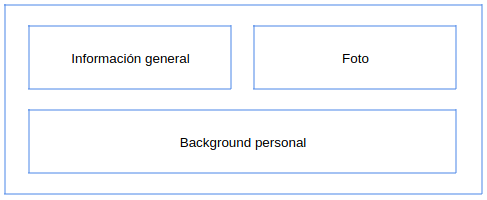
\includegraphics[width=0.5\textwidth]{Imagenes/Personas/Plantilla personas.png}
    \caption{Estructura de las personas}
    \label{fig:estructura-personas}
\end{figure}

\subsubsection{Marta González Torres}

\begin{minipage}{0.4\textwidth}
    \textbf{Información general} \\

    Edad: \textit{23 años} \\
    Sexo: Mujer \\
    Estudios: Ingeniería de Telecomunicaciones \\
    Gustos: Escuchar música e ir a conciertos cuando puede \\
\end{minipage}
\hfill
\begin{minipage}{0.4\textwidth}
    \centering
    
\includegraphics[width=0.5\textwidth]{Imagenes/Personas/Marta.jpg}
    \label{fig:fotoMarta}
    \captionof{figure}{Fotografía de Marta}
\end{minipage}

\textbf{Background personal} \\

Marta no puede salir de su casa sin los auriculares. Para ella la música es una gran parte
de su vida, y todas las mañanas, en la parada del bus, \textit{se prepara un playlist personalizada
en Spotify} para el itinerario hasta la Universidad. \textit{Vive en Fuenlabrada}, por lo que tiene
una ruta de una hora hasta que llega a Madrid, \textit{donde va a clase en la UCM}. \\ 

A Marta sobre todo le gusta la música italiana, ya que en el 2020 se fue de Erasmus a Turín y se
enamoró tanto de su cultura como de su música. Su cantante favorita es Francesca Michielin, así que
cuando hace gira intenta ir a algún concierto suyo en una \textit{ciudad italiana en la que no haya
estado}. De esta manera, puede conocer más la cultura italiana que tanto le gusta y sus diferenciados
a lo largo del país. \\

Se da la casualidad de que a su hermano Julián también le gusta mucho Francesca, así que en varias
ocasiones \textit{han ido ellos de viaje junto a sus padres} Carlos y Elena, los cuáles se van a
cenar juntos mientras sus hijos están en el concierto. \textit{Esto no lo hacen muy a menudo} debido
a que solo van cuando hay un concierto en alguna ciudad que les resulte interesante a toda la familia.
Normalmente se encarga ella de hacer la reserva tanto de los vuelos, \textit{para lo que usa
SkyScanner, como del alojamiento, utilizando AirBnB en este caso}. Esto se le hace a veces complicado
ya que quieren ir a varios sitios y tiene que cuadrar los horarios de todo. Por este motivo prefiere usar la 
aplicación web de las compañías, ya que así puede tener varias pestañas abiertas en las que visualiza toda
la información a la vez. \\

Con respecto al tema universitario, a Marta se le está haciendo cuesta arriba. Se metió inicialmente
en telecomunicaciones porque \textit{se le daban bien las matemáticas y la tecnología}, pero la
carrera no fue lo esperado. A pesar de las dificultades, la carrera le gusta y querría terminarla,
ya que este será en principio su último año. Pero estos problemas la agobian bastante, y para
distraerse le gusta mucho \textit{ir a festivales de música por España}. Suele ir todos los años
al festival Starlite, pues Pablo, el novio de su hermano y con el que mantiene muy buena relación,
es de Marbella, y se puede quedar algunos días en la playa aprovechando el viaje. Pero a pesar de
que no tiene que pagar gastos de alojamiento, el evento musical es bastante caro (ya que va varios
días), por lo que \textit{intenta ahorrar lo máximo posible en el viaje}. Para eso usa comparadores
de viaje como Omio, además de revisar las páginas de aerolíneas como \textit{RyanAir}, ya que a veces son
incluso más baratas que un vuelo o un tren.

\subsubsection{Isabel García Rodríguez}
\begin{minipage}{0.4\textwidth}
    \textbf{Información general} \\

    Edad: \textit{30 años} \\
    Sexo: Mujer \\
    Estudios: Psicología \\
    Gustos: Pintura y participar en grupos de apoyo para personas con discapacidad. \\
\end{minipage}
\hfill
\begin{minipage}{0.4\textwidth}
    \centering
    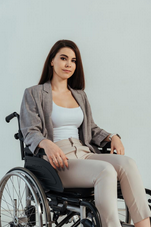
\includegraphics[width=0.5\textwidth]{Imagenes/Personas/Isabel.png}
    \label{fig:fotoIsaP}
    \captionof{figure}{Fotografía de Isabel}
\end{minipage}

\textbf{Background personal} \\

Isabel es una psicóloga comprometida con la mejora de la calidad de vida de las personas con discapacidad. \textit{Tiene una 
discapacidad física desde su nacimiento} que afecta su movilidad y requiere el uso de una silla de ruedas. Actualmente
\textit{vive en una pequeña urbanización a las afueras de Barcelona}. \\

Su familia vive en un pequeño pueblo de Huesca, por lo que \textit{siempre que puede se desplaza para verlos}. Muchas veces 
tiene el problema de la falta de autobuses que conectan con el pueblo, por lo que \textit{utiliza Omio, que realiza el trayecto
por ella, indicándole los transbordos que tiene que realizar y facilitándole la ayuda que necesita en todo momento}. \\

Ha asistido a varios cursos y conferencias relacionados con la psicología y la discapacidad, lo que la ha llevado a 
\textit{planear viajes a diferentes ciudades para participar en eventos}. Utiliza comparadores de viaje para encontrar opciones 
que se adapten a sus necesidades específicas, como hoteles con habitaciones adaptadas y \textit{vuelos con asistencia en el 
aeropuerto}. \textit{Algunos de los comparadores que usa no tienen opción de solicitar ayuda en caso de que tengas dudas, por lo que si
tiene algún problema no puede contactar con nadie}. Antes de realizar la reserva, ella sabe las distintas compañías y empresas que te lo suelen proporcionar. \\

Aparte de su trabajo, Isabel es una apasionada de la pintura y trata de visitar galerías y estudios de artistas en cada 
destino que visita. Isabel también es miembro activo de grupos de apoyo para personas con discapacidad en su ciudad. \textit{Allí 
es donde comparte experiencias y ofrece apoyo a otros miembros, por ejemplo a los jóvenes con discapacidad, para fomentar 
su independencia y autoestima}. Viaja a menudo con su mejor amiga, Carmen, quien la ha apoyado en su viaje de empoderamiento 
y ha aprendido mucho sobre la discapacidad en el proceso también.

\subsection{Validación de las personas}
Una vez finalizada la creación de las distintas personas (Marta e Isabel), vamos a pasar a validarlas. Para ello, vamos a comprobar dos cosas. La primera
de ellas es que toda la información contenida en los esqueletos se encuentre en las personas correspondientes y la segunda es que estas personas encapsulen
todos los factoides identificados en las listas. \\

Tras realizar una revisión de estas características, hemos notado que parte de la información que teníamos en las listas de factoides (que nos hemos dejado
o que ha sido añadida posteriormente) no se encontraba en los esqueletos y algunas características de los esqueletos que no se encontraban propiamente
redactadas en las personas. \\

Lo que falta bien sea en los esqueletos o en las personas es la siguiente información, que ya ha sido modificada en el lugar correspondiente:
\begin{itemize}
    \item Organiza sus viajes cuadrando los horarios para tener el mejor precio.
    \item Busca en las páginas de las aerolíneas.
    \item Se ha propuesto viajar más.
    \item Viaja en autobús.
    \item Viaja para conocer nuevas culturas y lugares.
    \item Prefiere la búsqueda en el ordenador antes que en el móvil.
    \item Viaja para ver a sus familiares.
    \item Nivel económico alto.
    \item Le parece complicado pedir ayuda dentro de la página.
    \item Necesitan en ocasicones que les desplacen.
    \item Conoce aquellas empresas que son más accesibles para las personas con discapacidad.
\end{itemize}

\subsection{Tipos de personas}
\begin{itemize}
    \item \textbf{Persona Primaria} - \textit{Marta González Torres (Viajero que usa comparadores de viajes)} $\rightarrow$ Representa al tipo de usuario consumidor de comparadores de viajes. Se tratan de usuarios que utilizan activamente las funcionalidades de los comparadores con el objetivo de ahorrar lo máximo posible en los transportes para sus viajes.
    \item \textbf{Persona Secundaria} - \textit{Isabel García Rodríguez (Viajero con discapacidad)} $\rightarrow$ Representa al tipo de usuario consumidor o no consumidor de comparadores de viajes que tienen una necesidad añadida o distinta al resto de usuarios. 
    Generalmente usuarios que aparte de la interfaz ya creada necesitaran de una pequeña adaptación visual o sensorial para poder sacar el máximo provecho a la aplicación. En el caso de Isabel necesitaría un apoyo extra debido a su discapacidad que presenta, ya que sus viajes esterían mucho más condicionados que los de Marta.
\end{itemize}